\chapter{Instalaciones necesarias}
Es necesario configurar el ambiente de  desarrollo con las siguientes herramientas :\\
\section{Node js.}
Instalaremos la versi\'on estable.Descargamos el instalador para windows desde :\\
\url{https://nodejs.org/es/}\\
\begin{figure}[H] % Ambiente 'figure'
	\centering % imagen sin escalar
	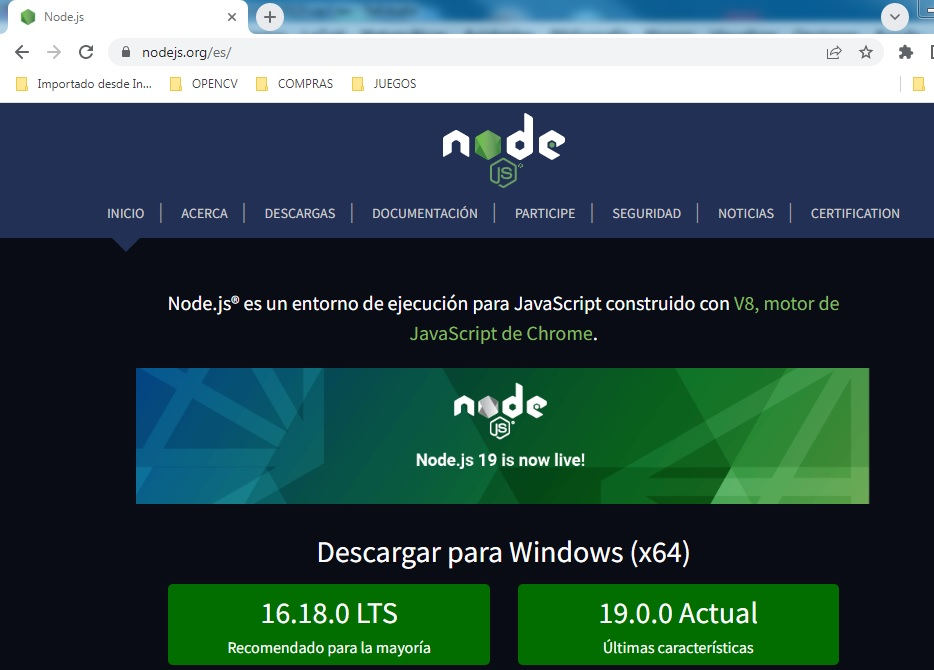
\includegraphics[scale=0.4]{images/c1_1.jpg}
	\caption{P\'agina de node js.}
\end{figure}
Verificamos las versiones de node que tenemos con los siguientes comandos en un cmd .\\
\texttt{node -v}\\
\texttt{npm -v}\\
\begin{figure}[H] % Ambiente 'figure'
	\centering % imagen sin escalar
	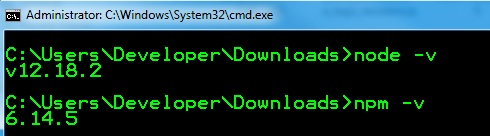
\includegraphics[scale=0.7]{images/c1_2.jpg}
	\caption{Versi\'on de node.}
\end{figure}
\section{NVM.}
Instalaremos la versi\'on estable.Descargamos el instalador para windows desde :\\
\url{https://github.com/coreybutler/nvm-windows/releases}\\
Al asistente de instalacion damos next,next.Una vez instalado, en un cmd en modo administrador ejecutamos :\\
\texttt{nvm v}\\
Para ver la lista de versiones node instaladas en nuestra PC/laptop.\\
\texttt{nvm list}\\
Instalamos una version de node.\\
\texttt{nvm install 16.0.0}\\
Para usar una version de node en especifico.\\
\texttt{nvm use 16.0.0}\\
Para desistalar una version de node.\\
\texttt{nvm unstall 16.0.0}\\

\section{TypeScript.}
Para instalar ejecutamos el siguiente comando.En un cmd en modo administrador\\
\texttt{npm install -g typescript}\\
Para ver la versi\'on :\\
\texttt{tsc -- version}\\
\begin{figure}[H] % Ambiente 'figure'
	\centering % imagen sin escalar
	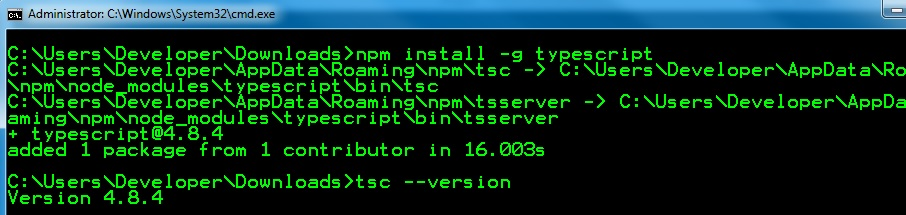
\includegraphics[scale=0.7]{images/c1_3.jpg}
	\caption{TypeScript y versi\'on.}
\end{figure}

\section{Angular Cli.}
Instalaremos el gestor de angular.Ejecutamos el siguiente comando en un cmd en modo administrador.Usaremos esta angular ya que es compatible con node 12\\
\texttt{npm install -g @angular/cli@12.0.0}\\
Para ver la versi\'on que tenemos:\\
\texttt{ng -v}\\
\begin{figure}[H] % Ambiente 'figure'
	\centering % imagen sin escalar
	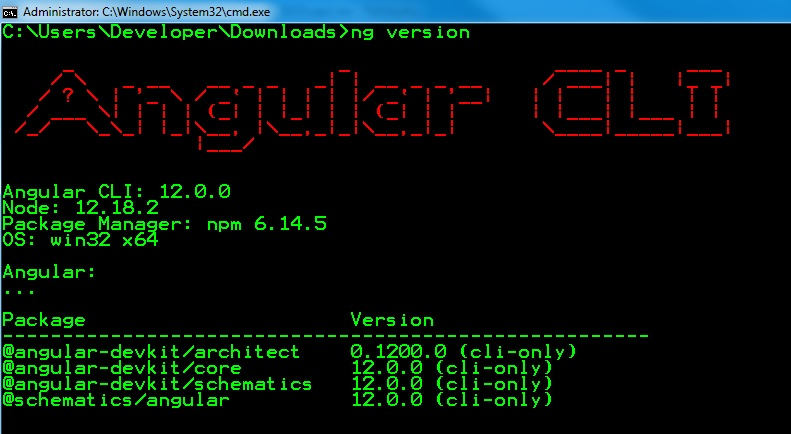
\includegraphics[scale=0.7]{images/c1_4.jpg}
	\caption{Angular y versi\'on.}
\end{figure}

\section{Ionic.}
Instalaremos el framework ionic.Ejecutamos el siguiente comando en un cmd en modo administrador.\\
\texttt{npm install -g ionic}\\
Para ver la versi\'on que tenemos:\\
\texttt{ionic -v}\\
\begin{figure}[H] % Ambiente 'figure'
	\centering % imagen sin escalar
	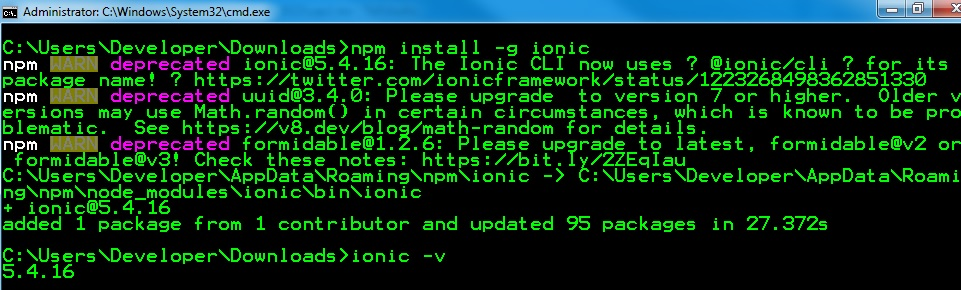
\includegraphics[scale=0.7]{images/c1_5.jpg}
	\caption{Ionic  y versi\'on.}
\end{figure}

\section{Visual Studio.}
Instalaremos  este editor de texto.Descargamos el instalador para windows desde :\\
\url{https://code.visualstudio.com/}\\\\
Instalaremos los siguientes plugins:
\begin{itemize}
	\item Angular 2 TypeScript Emmet.
	\item Angular 5 Snippets TypeScript, Html, Angular Material.
	\item Angular Language Service.
	\item Angular v5 Snippets.
	\item Angular2-inline.
	\item Bootstrap 4 Font Awesome snippets.
	\item HTML CSS Support.
	\item JavaScript (ES6) code snippets.
	\item JS-CSS-HTML FormatterJSHint.
	\item Material Icon Theme.
	\item Prettier Code Formatter.
	\item Terminal.
	\item TSLint.
	\item TypeScript Hero.
	\item TypeScript Importer.
\end{itemize}
Terminado el proceso, procedemos a cerrar y abrir de nuevo el editor de texto para que los cambios se apliquen.
\begin{figure}[H] % Ambiente 'figure'
	\centering % imagen sin escalar
	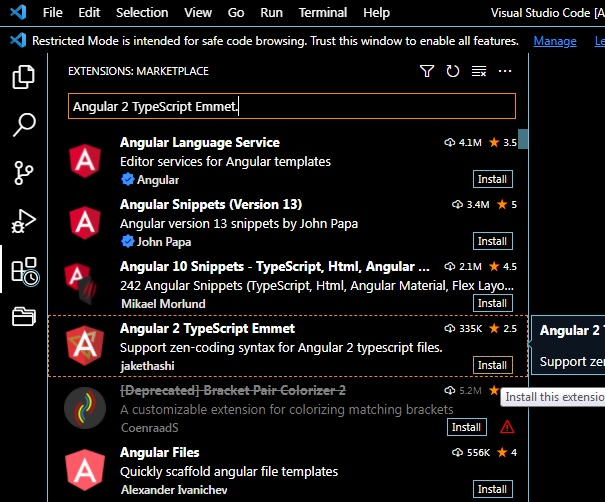
\includegraphics[scale=0.7]{images/c1_6.jpg}
	\caption{Visual Studio Code y plugins .}
\end{figure}








